\documentclass[11pt]{article}
\usepackage{graphicx}
\usepackage{float}
\usepackage{amsmath}
\usepackage{amsfonts}
\usepackage[brazilian]{babel}
\usepackage[utf8]{inputenc}
\usepackage[backend=biber]{biblatex}
\usepackage{csquotes}
%\usepackage{docmute}
\usepackage{array}
\usepackage[T1]{fontenc}

\newcommand{\fromeng}[1]{\footnote{do inglês: \textit{#1}}}
\newcommand{\tit}[1]{\textit{#1}}
\newcommand{\tbf}[1]{\textbf{#1}}
\newcommand{\ttt}[1]{\texttt{#1}}

\newcolumntype{C}[1]{>{\centering\let\newline\\\arraybackslash\hspace{0pt}}m{#1}}

\begin{document}

\begin{titlepage}
	\centering
	{\scshape\Large Relatório de Projeto\par}
	\vspace{1.5cm}
	{\huge\bfseries Um sistema de Chat com envio de arquivos\par}
	\vspace{1cm}
	{\itshape Erik de Godoy Perillo -- RA 135582\par}
	\vspace{0.5cm}
	\begin{abstract}
		Neste relatório, serão descritas as funcionalidades e decisões de
		implementação do sistema de Chat para a disciplina
		MC833 -- Laboratório de Redes.
	\end{abstract}
	\vfill
	Universidade Estadual de Campinas 
	\vfill
	{\large \today\par}
\end{titlepage}

\newpage

\tableofcontents

\newpage

\section{Introdução}
\paragraph{}
A aplicação é um sistema de chat cliente/servidor. 
São suportadas conversas entre dois usuários ou em grupos.
Pode-se também enviar/receber arquivos, com confirmação de recebimento.
Mensagens/arquivos enviados são guardados no servidor até que o usuário
destino esteja \tit{online} para recebê-las.
Os usuários que enviaram as mensagens/arquivos são notificados assim que
as mensagens são marcadas para envio e enviadas ao destino.

\section{Uso}
\subsection{Instalação}
\paragraph{}
Basta, do diretório raiz do projeto, entrar no diretório \ttt{src} e invocar
\ttt{make}. Não foram usadas bibliotecas adicionais além das padrão do C++14
e \ttt{pthread}.

\subsection{Execução}
\paragraph{}
É necessário primeiro ter o servidor rodando em algum lugar:

\ttt{\$ server <porta>}

Onde \ttt{<porta>} é o número da porta onde deseja-se servir.
Após isso, é só utilizar um cliente do \tit{chat}. Basta usar:

\ttt{\$ client <ip\_servidor> <porta\_servidor> <nome>}

Onde \ttt{<ip\_servidor>} é o IP do servidor do chat e \ttt{<porta\_servidor>} 
é a porta onde ele funciona. 
\ttt{<nome>} é o seu nome de usuário. 
Caso o nome de usuário ainda não exista e tudo ocorra bem, o servidor 
responderá com \ttt{OK}\@.

\subsection{Comandos disponíveis}
\paragraph{}
Os comandos disponíveis são os seguintes \:
(não são diferenciadas maiúsculas de minúsculas nos nomes dos comandos):
\begin{itemize}
	\item \ttt{help} -- Mostra uma mensagem com os comandos suportados.
	\item \ttt{send <usuario> <mensagem>}
		-- Envia ao usuário \ttt{<usuario>} a mensagem \ttt{<mensagem>}.
	\item \ttt{createg <nome\_grupo>}
		-- Cria um grupo nomeado \ttt{<nome\_grupo>}.
	\item \ttt{joing <nome\_grupo>}
		-- Entra no grupo \ttt{<nome\_grupo>}.
	\item \ttt{sendg <nome\_grupo> <mensagem>}
		-- Envia \ttt{<mensagem>} a todos os usuários do 
		grupo \ttt{<nome\_grupo>}.
	\item \ttt{sendf <usuario> <arquivo>}
		-- Envia o arquivo localizado em \ttt{<arquivo>} para o usuário
		\ttt{<usuario>}.
	\item \ttt{who} -- Lista todos os usuários do chat, assim como o 
		\tit{status} de cada um (\tit{online/offline}).
	\item \ttt{accept <usuario>:<arquivo>}
		-- Aceita o arquivo \ttt{<arquivo>} enviado por \ttt{<usuario>},
		se há algum.
	\item \ttt{exit} -- Sai do chat.
\end{itemize}

Para cada comando, a resposta do servidor é interpretada e é mostrado na tela
uma mensagem informativa sobre o que aconteceu.

\section{Detalhes de Projeto}
\paragraph{}
O projeto foi implementado usando-se a linguagem C++, lidando com os aspectos
de rede com bibliotecas da linguagem C e abstraindo seus detalhes.

\subsection{Arquitetura}
\paragraph{}
Foi escolhido para implementação do projeto a arquitetura 
MVC\fromeng{Model-View-Controller}, pela modularização que ela proporciona, 
que é muito adequada para lidar com sistemas onde há múltiplas iterações
ao mesmo tempo. 
A figura~\ref{fig:arq} ilustra a arquitetura geral do projeto e as iterações
que acontecem entre cada módulo.
\begin{figure}[H]
	\centering
	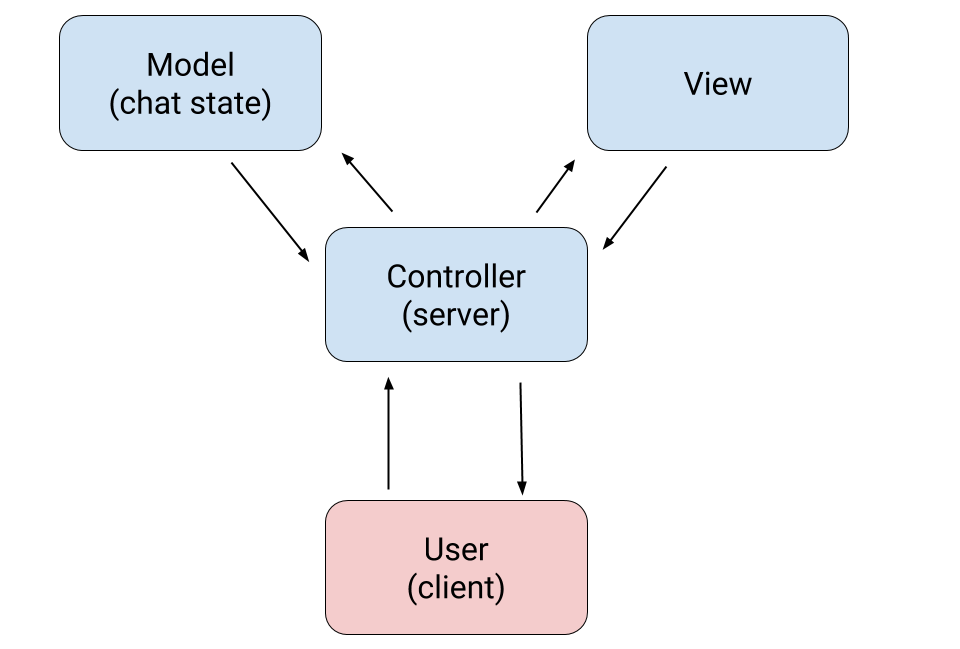
\includegraphics[width=0.8\linewidth]{imgs/mvc.png}
	\caption[7pt]{A arquitetura geral do projeto}
	\label{fig:arq}
\end{figure}

\subsubsection{Chat}
O componente \tit{model} do sistema é a classe \tit{Chat}, que mantém o tempo
todo o estado inteiro do chat. No modelo, há informações sobre:
\begin{itemize}
	\item \tbf{Usuários} -- Representados por uma classe \tit{User}, que contém
		informações sobre seu nome no chat e endereço da Internet
		(representado por uma classe \tit{NetAddr} que será discutida mais 
		a fundo em breve).
	\item \tbf{Grupos} -- Representados por uma classe \tit{Group}, que contém 
		informação sobre o nome do grupo e os usuários nele inseridos.
	\item \tbf{Mensagens} -- Representadas por uma classe \tit{Message}, que
		representa uma mensagem no chat, com seu usuário fonte, destino e o
		corpo da mensagem. Pode também representar um arquivo. Nesse caso,
		os bytes do arquivo são colocados no campo da mensagem. 
		Para o cálculo das funções \tit{hash}, usou-se uma especialização
		do método \tit{hash} provido pela biblioteca padrão do C++.
		Ela detecta se a mensagem em questão é uma mensagem comum ou um
		arquivo: se for uma mensagem comum, faz uma combinação usando
		o destino, fonte e mensagem. Se for um arquivo, faz a combinação
		usando o destino, fonte e o nome do arquivo.
\end{itemize}

Para se manter o estado dos usuários \tit{online} e \tit{offline}, simplesmente
cria-se grupos \tit{online} e \tit{offline} e, então, os usuários são
inseridos/removidos desses grupos conforme necessário.

A classe \tit{ChatView} é o componente \tit{View} do sistema. 
É através dela que se obtém representações visuais sobre o estado do chat. 
É por ela, por exemplo, que é construída a tabela de usuários do \tit{chat}
que é enviada para os clientes que a pedirem.

\subsubsection{Servidor}
\paragraph{}
O servidor do chat é composto de três tipos de \tit{threads} principais: 
\begin{itemize}
	\item \tbf{Despachadora} -- 
		Fica ouvindo por requisições de conexões novas
		e, caso a conexão se estabeleça e haja \tit{threads} disponíveis, 
		cria uma nova \tit{thread} de interação com o usuário novo.
	\item \tbf{Iteração com o usuário} -- 
		Permanece esperando por novas requisições de um certo usuário e,
		quando a recebe, toma a ação apropriada.
	\item \tbf{Manipulação de mensagens} --
		Checa continuamente por mensagens novas a serem enviadas. 
		Para cada mensagem na fila de envio, tenta enviar a mensagem para
		o destino e, em sucesso, notifica quem enviou a mensagem que ela
		foi entregue.
\end{itemize}
Desse modo, múltiplos clientes podem ser atendidos ao mesmo tempo (cada um com 
uma thread de interação dada pelo servidor) e as mensagens são manipuladas 
de forma assíncrona.

\subsubsection{Cliente}
\paragraph{}
O cliente é composto de duas \tit{threads}:
\begin{itemize}
	\item \tbf{Recebedora de comandos} --
		Essa thread continuamente recebe comandos do console e manda a 
		requisição apropriada ao servidor.
	\item \tbf{Notificações} --
		Nessa thread, fica-se escutando por mensagens do servidor e as ações
		necessárias são tomadas.
\end{itemize}

\subsection{Rede}
\paragraph{}
A comunicação entre usuários/servidor é toda feita através do protocolo TCP\@.
Tal protocolo foi escolhido para não haver a necessidade de lidar com
confirmação de recebimento de mensagens e recebimento de bytes fora de ordem.
Entretanto, ainda é necessário manipular os bytes que chegam pela conexão,
pois há um formato específico para as mensagens e o protocolo TCP não garante
que todos os bytes enviados por uma chamada a \ttt{send} serão recebidos 
da mesma forma pela chamada a \ttt{recv} do outro lado (pode acontecer, por
exemplo, de o último \tit{buffer} ser concatenado ao primeiro em uma chamada
a \ttt{recv} feita duas vezes -- Ainda em ordem, claro).

\subsubsection{Abstrações}
Foram feitas abstrações para todos os componentes importantes na comunicação
por rede a fim de facilitar seu uso por aplicações como o \tit{chat} e outras.
As principais abstrações foram feitas para:
\begin{itemize}
	\item \tbf{Endereços de rede} -- Foi criada uma classe \tit{NetAddr} que 
		representa um endereço de rede. Assim pode-se, por exemplo, instanciar
		um objeto \tit{NetAddr} passando-se apenas como parâmetros o 
		endereço IP e a porta, e a classe toma conta de preencher as estruturas
		como \ttt{sockaddr\_in} apropriadamente.
	\item \tbf{Mensagens entre \tit{Hosts}} -- 
		Por motivos citados acima, foi preciso
		criar um formato padronizado de mensagens a ser entendido por 
		cliente e servidor. Para representar isso, há a classe \tit{NetMessage},
		que contém uma mensagem em um formato padronizado (a ser discutido a
		seguir) com informações sobre destino e fonte.
		Para se receber tais mensagens, há uma classe \tit{NetReceiver},
		que faz chamadas repetidas a \ttt{send} e separa apropriadamente os
		bytes de forma a se obter mensagens no formato padronizado.
\end{itemize}

\subsubsection{Comunicação}
\paragraph{}
Toda mensagem a ser trocada por cliente e servidor tem o formato:

\ttt{CABEÇALHO <| CAMPO 1 | CAMPO 2 \dots>}

Onde os campos são opcionais. É necessário, ao menos, ter um cabeçalho, que
indica qual a mensagem que chegou. 
Esse cabeçalho tem sempre um \tit{byte}.
A codificação das mensagens é feita na biblioteca \ttt{protocol} criada 
para a aplicação.
A mensagem é sempre terminada com um caractere especial e, se há campos 
adicionais na mensagem, estes são separados por outro caractere especial.
Há funções que garantem que \tbf{toda} cadeia de caractere inserida nas 
mensagens é sanitizada, isto é, não há os caracteres especiais nelas.
Foram criadas funções especiais para cada mensagem. 
Ao usuário, só cabe passar os argumentos e a biblioteca cuida de garantir
com que a mensagem seja formatada adequadamente.
Após o recebimento da mensagem pelo outro lado, há outras funções que 
desmontam a mensagem e dão de volta a informação passada pelo usuário.

Como um exemplo, tomemos o caso de enviar uma mensagem para algum usuário
do \tit{chat}. 
O processo então é:
\begin{itemize}
	\item O usuário A digita em seu console o comando para enviar uma mensagem
		para o usuário B\@:

	\ttt{\$ send B MENSAGEM}
	\item O comando passa por \tit{parsing}, é identificado e é chamada
		uma função para montar a mensagem que vai ser transmitida pela rede,
		onde cada campo é sanitizado, a mensagem é montada e enviada pela rede:

	\ttt{msg = hostToNetSendMsg(A, B, MENSAGEM);}

	\item Do outro lado, o servidor recebe a mensagem, extrai o cabeçalho e 
		então chama \ttt{netToHostSendMsg(msg)}, que devolve um objeto da
		classe \ttt{Message} pronto para ser colocado na fila de mensagens.
\end{itemize}

\end{document}
